%%%%%%%%%%%%%%%%%%%%%%%%%%%%%%%%%%%%%%%%%%%%%%%%%%%%%%%%%%%%%%%%%%%%
%%%%%%%%%%%%%%%%%%%%%%%%%%%%%%%%%%%%%%%%%%%%%%%%%%%%%%%%%%%%%%%%%%%%
%%  Albert Abelló Lozano MSc Thesis document                                                               %%
%%%%%%%%%%%%%%%%%%%%%%%%%%%%%%%%%%%%%%%%%%%%%%%%%%%%%%%%%%%%%%%%%%%%
%%%%%%%%%%%%%%%%%%%%%%%%%%%%%%%%%%%%%%%%%%%%%%%%%%%%%%%%%%%%%%%%%%%%

%% K‰yt‰ toinen n‰ist‰, jos kirjoitat suomeksi:
%% ensimm‰inen, jos k‰yt‰t pdflatexia (kuvat on oltava pdf-tiedostoina)
%% toinen, jos haluat tuottaa ps-tiedostoa (k‰yt‰ eps-formaattia kuville).
%%
%% Use one of these you write in Finnish:
%% the 1st when using pdflatex (use pdf figures) or
%% the 2nd when producing a ps file (use eps figures).
%\documentclass[finnish,12pt,a4paper,pdftex]{article}
%\documentclass[finnish,12pt,a4paper,dvips]{article}


%% K‰yt‰ n‰it‰, jos kirjoitat englanniksi
%%
%% Uncomment one of these if you write in English
\documentclass[english,12pt,a4paper,pdftex]{article}
%\documentclass[english,12pt,a4paper,dvips]{article}

%% T‰m‰ paketti on pakollinen
%% Valitse korkeakoulusi n‰ist‰: arts, biz, chem, elec, eng, sci.
%%
%% This package is required
%% Choose your school from arts, biz, chem, elec, eng, sci.
\usepackage[elec]{aaltothesis}

%% Jos k‰yt‰t latex-komentoa k‰‰nnett‰ess‰ (oletusarvo) 
%% kuvat kannattaa tehd‰ eps-muotoon. ƒl‰ k‰yt‰ ps-muotoisia kuvia!
%% K‰yt‰ seuraavaa latex-komennon ja eps-kuvien kanssa 
%%
%% Jos t‰‰s k‰yt‰t pdflatex-komentoa, joka k‰‰nt‰‰ tekstin suoraan
%% pdf-tiedostoksi, kuvasi on oltava jpg-formaatissa tai pdf-formaatissa.
%%
%% Use this if you run pdflatex and use jpg/pdf-format pictures.
%%
\usepackage{graphicx} 
\graphicspath{{../figures/}}
%%\DeclareGraphicsExtensions{.pdf}{png}{.png}{.jpg}{jpg}{.jpeg}{jpeg}
\DeclareGraphicsExtensions{.pdf}
\usepackage{url}
\usepackage[small, bf]{caption}
\usepackage[font=small]{subfig}
\usepackage{ucs} % Soporte Unicode
\usepackage[utf8x]{inputenc} % Ficheros de entrada en latin1
%% Use this if you do not like hyperref package - this
%% defines url environment and formats it correctly

%% Matematiikan fontteja, symboleja ja muotoiluja lis‰‰, n‰it‰ tarvitaan usein 
%%
%% Use this if you write hard core mathematics, these are usually needed
\usepackage{amsfonts,amssymb,amsbsy}  

%% Vaakasuunnan mitat, ƒLƒ KOSKE!
\setlength{\hoffset}{-1in}
\setlength{\oddsidemargin}{35mm}
\setlength{\evensidemargin}{25mm}
\setlength{\textwidth}{15cm}
%% Pystysuunnan mitat, ƒLƒ KOSKE!
\setlength{\voffset}{-1in}
\setlength{\headsep}{7mm}
\setlength{\headheight}{1em}
\setlength{\topmargin}{25mm-\headheight-\headsep}
\setlength{\textheight}{23cm}


%% Kaikki mik‰ paperille tulostuu, on t‰m‰n j‰lkeen
%%
%% Output starts here
\begin{document}

%% Korjaa vastaamaan korkeakouluasi, jos automaattisesti asetettu nimi on 
%% virheellinen 
%%
%% Change the school field to describe your school if the autimatically 
%% set name is wrong
% \university{aalto University}{aalto-Yliopisto}
% \school{School of Electrical Engineering}{S‰hkˆTekniikan korkeakoulu}

%% Vain kandityˆlle: Korjaa seuraavat vastaamaan koulutusohjelmaasi
%%
%% Only for B.Sc. thesis: Choose your degree programme. 
\degreeprogram{Electronics and electrical engineering}%
{Elektroniikka ja s‰hkˆtekniikka}
%%

%% Vain DI/M.Sc.- ja lisensiaatintyˆlle: valitse laitos, 
%% professuuri ja sen professuurikoodi. 
%%
%% Only for M.Sc. and Licentiate thesis: Choose your department,
%% professorship and professorship code. 
\department{Department of Communication and Networking}%
{Radiotieteen ja -tekniikan laitos}
\professorship{Networking Technology}{Piiriteoria}
\code{S-55}
%%

%% Valitse yksi n‰ist‰ kolmesta
%%
%% Choose one of these:
%\univdegree{BSc}
\univdegree{MSc}
%\univdegree{Lic}

%% Oma nimi
%%
%% Should be self explanatory...
\author{Albert Abell\'o Lozano}

%% Opinn‰ytteen otsikko tulee vain t‰h‰n. ƒl‰ tavuta otsikkoa ja
%% v‰lt‰ liian pitk‰‰ otsikkoteksti‰. Jos latex ryhmittelee otsikon
%% huonosti, voit joutua pakottamaan rivinvaihdon \\ kontrollimerkill‰.
%% Muista ett‰ otsikkoja ei tavuteta! 
%% Jos otsikossa on ja-sana, se ei j‰‰ rivin viimeiseksi sanaksi 
%% vaan aloittaa uuden rivin.
%% 
%% Your thesis title. If the title is very long and the latex 
%% does unsatisfactory job of breaking the lines, you will have to
%% break the lines yourself with \\ control character. 
%% Do not hyphenate titles.
\thesistitle{Performance analysis of WebRTC}{Opinn‰yteohje}

\place{Espoo}
%% Kandidaatintyˆn p‰iv‰m‰‰r‰ on sen esitysp‰iv‰m‰‰r‰! 
%% 
%% For B.Sc. thesis use the date when you present your thesis. 
\date{20.3.2012}

%% Kandidaattiseminaarin vastuuopettaja tai diplomityˆn valvoja.
%% Huomaa titteliss‰ "\" -merkki pisteen j‰lkeen, 
%% ennen v‰lilyˆnti‰ ja seuraavaa merkkijonoa. 
%% N‰in tehd‰‰n, koska kyseess‰ ei ole lauseen loppu, jonka j‰lkeen tulee 
%% hieman pidempi v‰li vaan halutaan tavallinen v‰li.
%%
%% B.Sc. or M.Sc. thesis supervisor 
%% Note the "\" after the comma. This forces the following space to be 
%% a normal interword space, not the space that starts a new sentence. 
\supervisor{Prof.\ J\"org Ott}{Prof.\ J\"org Ott}

%% Kandidaatintyˆn ohjaaja(t) tai diplomityˆn ohjaaja(t)
%% 
%% B.Sc. or M.Sc. thesis advisors(s). 
%%
%% Note that there has been a change in the official EN translation
%% of the Finnish title ``ohjaaja'' which in the previous version (1.5) 
%% of this document was called ``instructor''. The recommended
%% translation is now ``advisor''.  
%% However, the LaTeX internal variable remains \instructor
%% as there is little point to change the variable name. 
%%
%\instructor{Prof. Pirjo Professori}{Prof. Pirjo Professori}
\instructor{M.Sc.\ (Tech.) Varun Singh}{TkT Varun Singh}
%\instructor{M.Sc.\ (Tech.) Polli Pohjaaja}{DI Polli Pohjaaja}

%% Aaltologo: syntaksi:
%% \uselogo{aaltoRed|aaltoBlue|aaltoYellow|aaltoGray|aaltoGrayScale}{?|!|''}
%% Logon kieli on sama kuin dokumentin kieli
%%
%% Aalto logo: syntax:
% \uselogo{aaltoRed|aaltoBlue|aaltoYellow|aaltoGray|aaltoGrayScale}{?|!|''}
%% Logo language is set to be the same as the document language.
\uselogo{aaltoRed}{''}

%% Tehd‰‰n kansilehti
%%
%% Create the coverpage
\makecoverpage

%% Pakotetaan uusi sivu varmuuden vuoksi, jotta 
%% mahdollinen suomenkielinen ja englanninkielinen tiivistelm‰
%% eiv‰t tule vahingossakaan samalle sivulle
%%
%% Force new page so that English abstract starts from a new page
\newpage
%
%% English abstract, uncomment if you need one. 
%% 
%% Abstract keywords
\keywords{Resistor, Resistance,\\ Temperature}
%% Abstract text
\begin{abstractpage}[english]
 Your abstract in English. Try to keep the abstract short, approximately 
 100 words should be enough. Abstract explains your research topic, 
 the methods you have used, and the results you obtained.  
\end{abstractpage}
%% Note that 
%% if you are writting your master's thesis in English place the English
%% abstract first followed by the possible Finnish abstract


%% Preface
\mysection{Preface}
Thank you everybody.\\

\vspace{5cm}
Otaniemi, 9.3.2012

\vspace{5mm}
{\hfill Albert Abell\'o Lozano \hspace{1cm}}

%% Pakotetaan varmuuden vuoksi esipuheen j‰lkeinen osa
%% alkamaan uudelta sivulta
%%
%% Force new page after preface
\newpage

%% Sis‰llysluettelo
%% addcontentsline tekee pdf-tiedostoon viitteen sis‰llysluetteloa varten
%% 
%% Table of contents. 
\addcontentsline{toc}{section}{Contents}


%% Tehd‰‰n sis‰llysluettelo
%%
%% Create it. 
\tableofcontents
\listoffigures
\listoftables

%% 
%% Corrects the page numbering, there is no need to change these
\cleardoublepage
\storeinipagenumber
%%
%%Definitions and abreviations
\mysection{Definitions and abreviations}
%\addcontentsline{toc}{section}{Definitions and abreviations}

\newpage

\pagenumbering{arabic}
\setcounter{page}{1}

%% 
%% Leave first page empty
\thispagestyle{empty}



%%introduction chapter
\section{Introduction}

%% 
%% Leave first page empty
\thispagestyle{empty}

The need of a new way to communicate between two points of the planet is a problem that many different technologies have tried to approach. Systems such Skype or VoIP are not able to cope the needs of the new generations of developers and users that everyday require a more integrated way of communication with the World Wide Web (WWW). 

Besides this, the amount of data transferred during the last years and the prevision for the future allocates a new scenario where non-centralized systems such as P2P are required as data bandwidth grows and systems need to become more scalable. Nowadays, networks are still manly content-centric, meaning that data is provided from a source to a client in a triangle scheme, clients upload data to central servers and this data is transferred to the endpoint. This architecture has been provided since long time as reliable and scalable, but with the appearance of powerful applications and Video On Demand (VOD) scalability is becoming an issue.

Those circumstances lead to a whole new world of real-time browser based applications which require also a new framework to work with. Ranging from online videoconferencing to real-time data applications, for this purpose few attempts were made in the past being highly reliable on specific hardware and custom-built no-compatible systems. Those proposals were not accessible to normal users that could not afford to adapt the requirements. 

All previous concepts are now possible thanks to the increase of the average performance in every computer nowadays, this situation is helping to build more complex browsers that are able to perform many different tasks that enhance web browsing to a different level. Having a browser to handle OpenGL style of applications is now possible thank to the new  HyperText Markup Language version 5 (HTML5) standard. Multimedia abilities are also able to be reproduced on those browsers and webcam media shown as HTML is now a reality. Even dough, there is still an important issue that must be addressed: there is no common standardized protocol that allows developers to do this. Web Real-Time Communication (WebRTC) effort to approach this problem is to build a simple and standard solution for peer-to-peer browser communication in the HTML5 environment~\cite{alvestrandOverview2012} .

Internet bandwidth capabilities helped to take the decision to start integrating peer-to-peer solutions in browsed based applications, this is due the year-by-year increase of user bandwidth connectivity during the last 10 years. Actual latency in the network is low enough to allow real-time applications to work resiliently in the browser. The amount of users being able to transfer at high speed has increased during last years (Figure~\ref{fig:bwWorldAvg}), about 39\% of users are able to download at speeds greater than 4Mbps being this a very good average speed for multimedia content~\cite{akamaiq2}.

\begin{figure}[h]
  \centering
    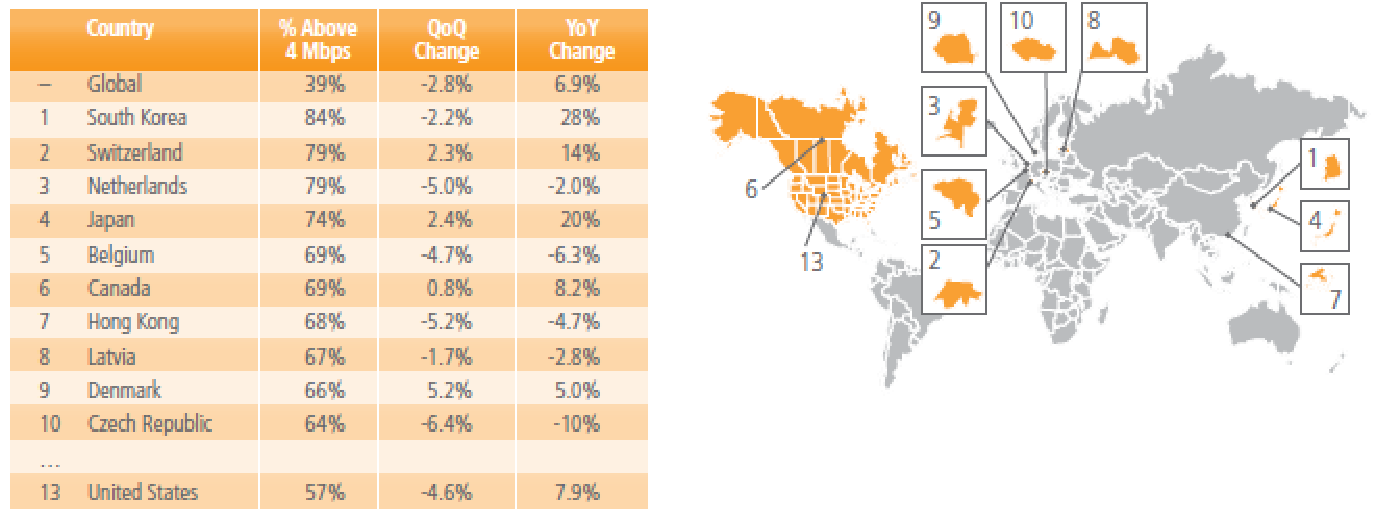
\includegraphics[width=1\textwidth]{./figures/internetstats.pdf}
      \caption[Broadband over 4Mbps connectivity statistics]{Broadband connectivity statistics about the speeds over 4Mbps around the globe.}
	\label{fig:bwWorldAvg}
\end{figure}

Regarding the specs on the client side, recent surveys and statistics taken by the game manufacturer Steam prove that more than  61\% of machines are carrying 1 to 4 gigabytes of RAM and nearly 90\% of computers handle 2 to 4 core CPU with a 64 bit OS~\cite{steamStats}, this environment can easily handle media enhanced applications that require high performance for media encoding. WebRTC concept rests over multiple layers having the browser as an underlying application, a traditional browser allocates a lot of resources for running being the performance of the machine a bottleneck in some cases.

Traditionally, WebRTC concept approaches rely on the usage of plug-ins or other separate software components that make the system run smoother by avoiding one layer of processing (browser) but being non-standard and not cross-compatible, one of the most import ant concepts when designing applications nowadays. This approach has a new alternative with the arrival of the new HTML5 where WebRTC is integrated as one of the new Application Programming Interfaces (APIs) available alongside other many different interesting capabilities.

\subsection{Background}

WebRTC API is included into the HTML5, this is the fifth version of the WWW language. This version includes different API's and JavaScript codes that help the developer to easily introduce new features into their already existing WWW applications. The initial HTML version (2.0) was published in November 1995 with the only goal of delivering static content from the server to client browser~\cite{html2IETF}. HTML became de de facto format for serving web information. 

HTML is written in tag formatting to identify different elements. Those tags are then interpreted by the browser to show the different data content served by the server. During the evolution of the WWW different new features have been added to the HTML standard and new versions where published, things like JavaScript and Style Sheets increase the flexibility and features of the WWW content enhancing the final user experience.

Due to the need to extend the features of the already existing HTML4 standard, a new version was proposed in 2004 by the Mozilla Foundation and Opera Software~\cite{initialHTML5proposition}. This new proposition focused in new developing technologies that could be backwards compatible with the already existing browsers, the idea didn't make a success and was tier apart until January 2008 when the first Public Working Draft was published by the Web HyperText Application Technology Working Group (WHATWG) in the W3C~\cite{firstHTML5draft}.

This proposal had a greater reliance in modularity in order to move forward faster, this meant that some specs that were included in the initial draft moved to different working groups in the W3C. Those technologies defined in HTML5 are now in separate specifications, one of them being WebRTC. WebRTC works as an integrated API within the browser that is accessible using JavaScript and is used in conjunction with the Document Object Model (DOM) interfaces. Some of the APIs that have been developed are not part of the HTML5 W3C specification but are included into the WHATWG HTML specification.

\subsection{Challenges}

WebRTC is a real time media protocol that will be obliged to share the available resources with many other applications. Due to the short experience in WebRTC congestion situations that share the available bandwidth with other existing solutions we will find some lack of documentation or previous literature regarding this topic. 

The aim to investigate and help to develop new protocols such as WebRTC is usually backed by a lack of information that may affect some of the statements made in this thesis. Hopefully, this won't affect the development of itself and the conclusions obtained at the moment of the development of the topic. 

Considering WebRTC is being developed at the moment of writing this thesis some of the statements made in here might be different in the following versions of WebRTC meaning that the problems analyzed have been solved.

\subsection{Contribution}

Investigate how WebRTC performs in a real environment trying to evaluate the best way to set multiple peer connections able to transfer media in different network topologies. Measure the performance of WebRTC in a real environment, identifying bottlenecks related to encoding/decoding, media establishment or connection maintenance. All this should be performed in real-time over a browser by using the already existing WebRTC API.

Using metrics related to RTT, latency, packet loss and bandwidth usage we expect to understand the way WebRTC performs when handling in different environments.

\subsection{Goals}

WebRTC uses and adapts some existing technologies for real-time communication. This thesis will focus in studying how:

\begin{itemize}
	\item WebRTC performs considering different topologies using video/audio acquired form the Webcam using the API and encoded using different codec types provided by the standard.

	\item Usage of WebRTC to build a real application that can be used by final users proving that the API is ready to be deployed and is a good approach for the developer needs when building real-time applications over the web. This will be done in conjunction with other new APIs and technologies introduced with HTML5.
	
	\item Testing of different WebRTC topologies with different network constraints to observe the response of the actual existing API.
\end{itemize}

The final conclusion will cover an overall opinion and usage experience of WebRTC, providing some valuable feedback for the needs and requirements for further modifications on the API.

\subsection{Structure}

Not sure about here

%documentation and drafts
%\section{Documentation and drafts}

%% 
%% Leave first page empty
\thispagestyle{empty}

Blah blah blah talk about the sdtrz process and APIs maybe? JSEP vs ROAP? CU-RTC-Web vs WebRTC? VP8 vs H.264 vs Optus? possible stuff to talk that might be interesting to introduce. Short and fast.

\subsection{CU-RTC-Web vs WebRTC}
In August 2012 Microsoft introduced his vision of a real-time communication between browser trying to cover all the WebRTC use cases with a different design \cite{curtcweb}, this draft collided directly with the ongoing WebRTC proposal done by the W3C working group \cite{webrtcW3cgroup}. W3C working group decided to attach to the already existing draft some aspects from the Microsoft proposal should be analyzed in comparison with WebRTC. Three main aspects differ from WebRTC:
\begin{itemize}
	\item No PeerConnection object
	\item No SDP description or JSEP
	\item No mantatory codec to be implemented
\end{itemize}
The ongoing WebRTC proposal identifies a Javascript object called RTCPeerConnection that handles and maintain all the peer connection data transfer, this object handles all the ICE, SDP creation, negotiation and transfer. In the CU-RTC-Web this concept is replaced with a proposal called RealtimeTransport interface that relies in a RemoteRealtimePort interface \cite{realtimemedia}. This design is a low-level API that forces web developers to build their own application-specific JavaScript code so it can be adapted to every different use case required. No API defined object like in WebRTC, more flexible but much more complicated to implement for application developers.

From the codec perspective CU-RTC-Web approach could be more sensitive to the codec war taking part on the workgroups, one of the key issues in the WebRTC standaritzation, not setting any codec to be mandatory makes sense considering that after long time there is no consensus about this position yet. On the other hand, it makes sense to set a mandatory codec for a media standard as it will force all the providers to set the same codec and avoid compatibility issues. Codecs being proposed are: VP8, H.264, Optus and G.711.

WebRTC draft RTCPeerConnection relies on a new Javascript spec called Javascript Session Establishment Protcol (JSEP) which help developers to handle the low-layer communication and negotiation tasks \cite{jsepIETF}. JSEP relies directly on the Session Description Protocol (SDP) \cite{sdpIETF}. CU-RTC-Web leaves freedom to developers to implement their own communication tasks for their specific application.

The conclusion shows that meanwhile WebRTC moves a lot of work to be done by the browser itself CU-RTC-Web leaves complete freedom to developers to adapt the use case to the proposal instead of adapting the application to the API such as in WebRTC. Both approaches can be valid, but WebRTC makes more sense form the developer point-of-view and it makes it easier to build applications on top of it.

\section{What is WebRTC?}

%% 
%% Leave first page empty
\thispagestyle{empty}

Web Real-Time Communication that builds P2P applications by using a defined API. The first announcement went public in a WG of the World Wide Web Consortium (W3C) in May 2011 \cite{webrtcW3cgroup} and started the official mailing list in April 2011 \cite{welcomeW3C}. During the first stage of discussion, the main goal was to define a public draft for the version 1 API implementation and a route timeline with the goal to publish the first version by March 2013. The first public draft of W3C came public the 27th of October 2011 \cite{originalW3Cdraft}. During this first W3C draft, only media (audio and video) could be sent over the network to other peers, it is focused in the way browsers are able to access the media devices without using any plugin or external software.

Alongside to the W3C working group, the WebRTC project also joined the IETF with a WG in May 2011 \cite{webrtcIETFgroup} with the first public announcement charter done the 3th of May 2011 \cite{webrtcIETFcharter}. Milestones of the WG initially marked December 2011 as deadline to provide the information and elements required to the W3C for the API design input. On the other side, the main goals of the WG covered the definition of the communication model, session management, security, NAT traversal solution, media formats, codec agreement and data transport \cite{webrtcIETFcharter}.

One  of the most important steps during the process of standardization came the 1st of June 2011 when Google publicly released the source code of their API implementation \cite{haraldpublicWebRTC}. 

During all this period both WGs have been working alongside to provide a reliable solution to enable cross-platform applications to perform media and data P2P transfer over the browser in a plugin-free environment. The first final version of the WebRTC API is to be published during March 2013.

\subsection{Support}

The following companies have supported and are actively working in the development of WebRTC standard in the W3C: Google, Mozilla and Opera \cite{googleAnnouncement}. Other companies such as Microsoft have supported browser-to-browser solution but have published their own proposal which differs with the one published in the WebRTC WG, called CU-RTC-Web \cite{curtcweb}, this proposal did not get much traction by the workgroup being declined to unify with the current specs, during an W3C workgroup poll in September 2012 the chairs of the group decided to attach to the already existing WebRTC API instead of moving it to the CU-RTC-Web \cite{curtcpoll}.

During the firsts attempts to build a reliable solution for WebRTC Ericsson Labs presented an initial API based on the preliminary work done in the WHATWG, this API was called ConnectionPeer API and required an special module to be installed in your browser \cite{ericssonwebrtc}. Ericsson lately dropped from the effort to build it's own browser to focus in the standardization and codec discussion, leaving the API implementation to the Mozilla and Chrome teams. The original API evolved rapidly during the next months thanks to the WGs and the developer community feedback that is experimenting with the unstable API.

\subsection{Milestones}

During the process of standardization some important moments should be remarked. In January 2012 Opera implemented the first version of WebRTC getUserMedia for accessing the camera and audio \cite{operaannouncement}, during this year getUserMedia is available in the stable version of Opera. 

Google Chrome integrated the first version of WebRTC in its DEV and Canary channels of the browser during January 2012 \cite{chromeannouncement}, in June 2012 it started moving its API to the stable channel hidden behind a flag, in November 2012 WebRTC becomes fully available in Google Chrome stable channel and is open for public usage \cite{chromestable}. 

Mozilla Firefox started working on the getUserMedia implementation early 2012 delivering the first version of media access trough API at the beginning of 2012 in the alpha version \cite{mozillablog}, in April 2012 Mozilla published a WebRTC video demo running on Firefox in the "adler" channel \cite{mozillawebrtc}, also supporting some primitive DataChannel API. Later in October Firefox Nightly was carrying the first unstable version of the WebRTC API including DataChannel \cite{mozillafinal}, Mozilla announced in September 2012 that the stable version of WebRTC will be shipped along with Firefox 18 in January 2013 \cite{mozillacomming}. 

Some announcements done from Microsoft point out that they are also working in some implementation into Internet Explorer by using CU-RTC-Web as the default standard, at the moment only the Media API information is publicly available \cite{microsoftcapture}.

In October 2012 Ericsson announced the world's first WebRTC-enabled browser for mobile devices called "Bowser" with support for iOS and Android, this browser is able to handle WebRTC calls using RTCWeb Offer/Answer Protocol (ROAP) which is an old discontinued version of the WebRTC API that has moved to Javascript Session Establishment Protocol (JSEP). This browser also differs from the previous desktop alternatives on the codec side, it is carrying H.264 for video and G.711 for audio \cite{ericssonbowser}. The API provided by Bowser is not fully W3C compliant.

\subsection{Alternatives}

Some alternatives are available to the WebRTC concept, considering the global architecture of WebRTC, Session Initiation Protocol (SIP) and Secure Real-Time Media Flow Protocol (RTMFP) are similar approaches to the same solution.

\subsubsection{SIP}

Both SIP and RTMFP are protocols to allow communication between two different users with audio/video support. SIP is an open standard and RTMFP is a proprietary protocol by Adobe, both systems are widely used for real-time communication. SIP final Request for Comments (RFC) was published in June 2004 \cite{sipRFC}, this chapter describes the methods and behaviors of SIP. From an overview perspective, SIP is an application-layer control protocol for multimedia sessions, can establish, maintain and terminate them, during the development of the standard different new functionalities were added to the drafts such as conferencing and the possibility of adding/removing media from existing sessions. SIP differentiates from RTMFP/WebRTC by locating the end user to be used for communication, this feature allows SIP to be closely related to traditional PSTN networks as it allow cross-domain communication which is not possible when using RTMFP/WebRTC. SIP is not a complete toolkit for communications, it works alongside with other existing protocols such as Real-time Transport Protocol (RTP), Real-Time Streaming Protocol (RSTP), Session Description Protocol (SDP) and Media Gateway Control Protocol (MEGACO). Using SDP for the session negotiation between the end-points and RTP/RSTP for the media transport, all those protocols usage is widely extended in the network and provides legacy for older technologies. Meanwhile SIP can locate and deliver a message to a user, SDP can provide the required information for the session establishment and RTP can transport the type of media specified in the SDP body.

\begin{figure}[h]
  \centering
    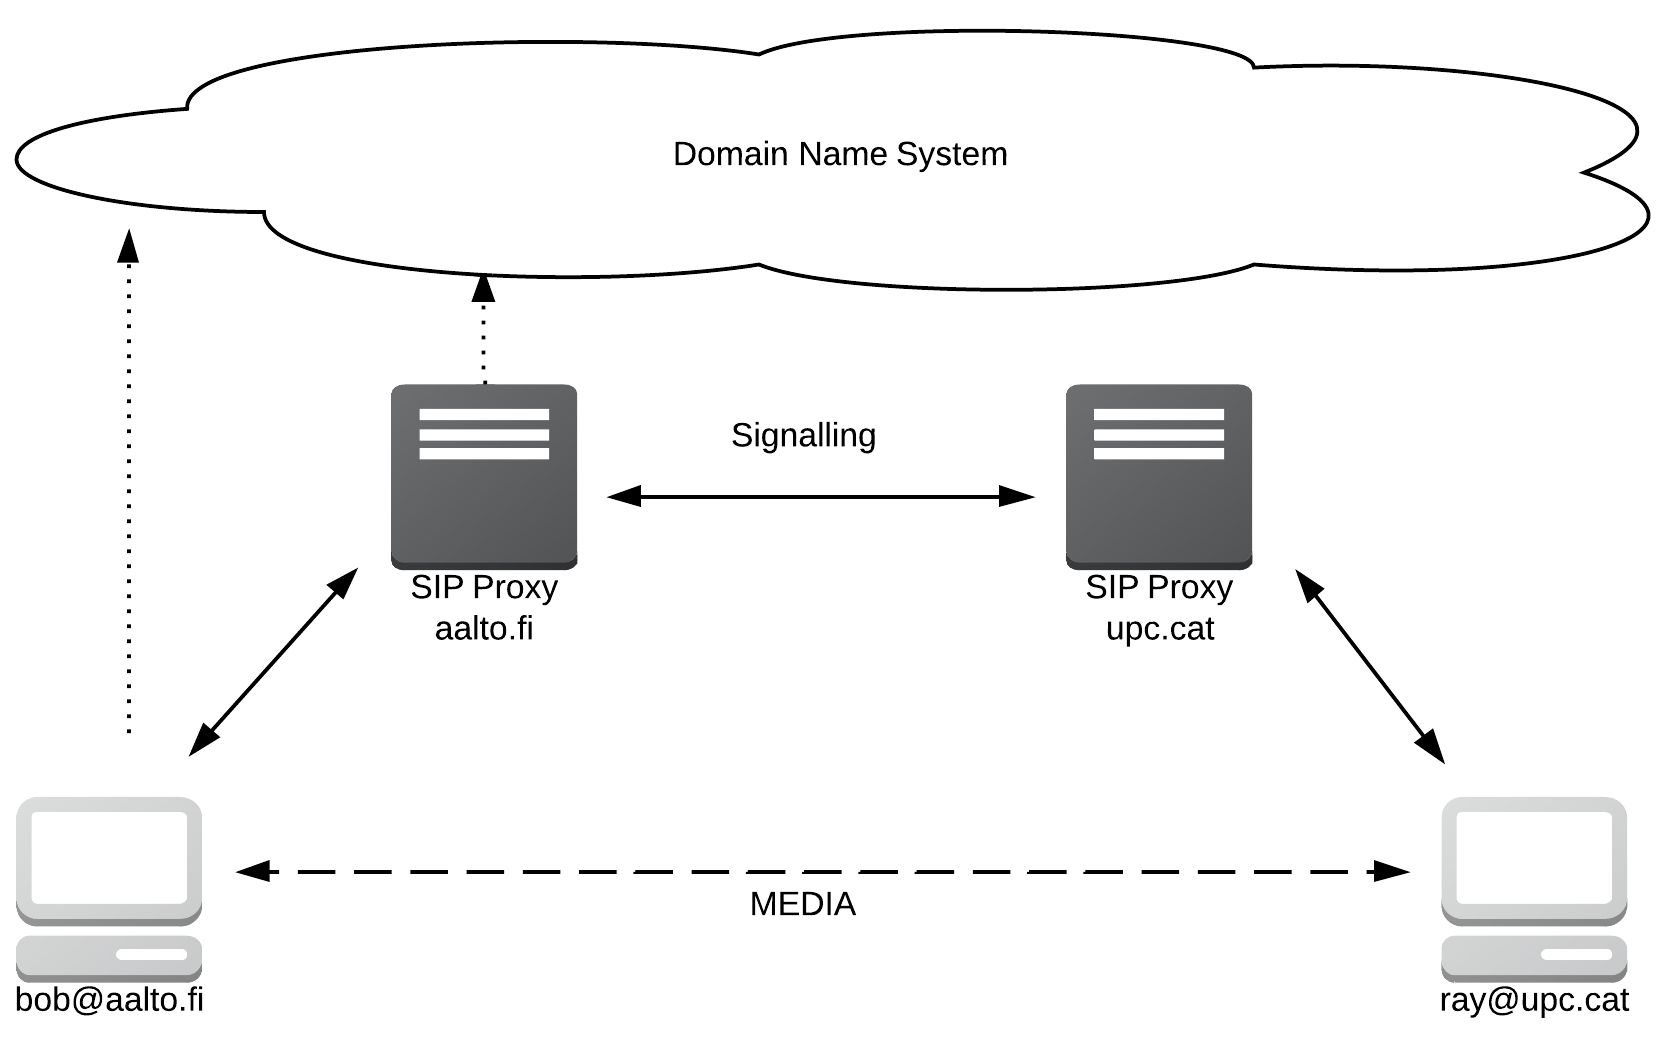
\includegraphics[width=1\textwidth]{./figures/SIParchitecture.png}
      \caption[SIP architecture for end-to-end signaling]{SIP architecture for end-to-end signaling.}
	\label{fig:SIParchitecture}
\end{figure}

SIP architecture relies in a trapezoid form where the Domain Name System (DNS) is used to locate the other peers of the system, once that peer is located and session is negotiated, media flows peer-to-peer directly to the endpoint. In order to build this system different agents are needed, SIP Proxies, SIP Redirect and SIP Registrar. SIP Proxies transmit the SDP and SIP messages from one peer to the other to establish communication (Figure ~\ref{fig:SIParchitecture}). SIP Registrar are the machines that collect and save all the user information from the end points.

DNS provides the IP address for both proxy servers and allow the messages to be exchanged between both peers, when SIP is used the following messages are exchanged: INVITE, RINGING and 200OK. Those messages carry the SDP data inside in an object format, when ray@upc.cat receives the INVITE message from bob@aalto.fi builds the 200OK response carrying the SDP object that providing compatibility check between both peers and which options and codecs to use. SIP provides some more messages to update the already existing session or to close them. The media transport is done using RTP and RTCP that rely over User Datagram Protocol (UDP) \cite{sipRFC}.

SIP is a pure Voice Over IP (VoIP) confederated technology that helped the community to learn about real-time P2P communication,we have used all the concepts and technologies embedded in SIP to build WebRTC.

\subsubsection{RTMFP and Adobe Flash}

RTMFP and Adobe Flash are proprietary technologies provided by Adobe, both services work together to provide multimedia and real-time communication between users.

Adobe Flash is a multimedia software that uses a plugin to work over the browser, it is used to build multimedia experiences for end users such as graphics, animation, games and Rich Internet Applications (RIAs). It is widely used to stream video or audio over webpages, in order to reproduce this content we need to install Adobe Flash plugin in our computer. It also carries different programming languages that drops from the standards called JavaScript Flash Language (JSFL) and ActionStript. Due to the need of using a plugin his extension to tablets and mobile devices is more complicated than using standards. Adobe Flash Player is available in most platforms except iOS devices and reaches about 98 of all internet-enabled desktop devices. This plugin allows developers to access media streams from external devices such as cameras and microphones to be used along with RTMFP.

RTMFP uses Adobe Flash to provide media and data transfer between two end points. This system usually works over UDP \cite{rtmfpDraft}. Differing from SIP, this protocol is a full suite for media/data transfer in a P2P constraint environment and carries its own signaling methods and codecs. It also handles congestion control on the packets and NAT transversal issues. One of the biggest differences is that, similar to WebRTC, is not a full communication infrastructure and both peers must be in the same working domain to be able to communicate, is not a PSTN style of communication but a point to point messaging system. This protocol is implemented in Flash Player, Adobe Integrated Runtime (AIR) and Adobe Media Server (AMS)  \cite{rtmfpDraft}, it is used for P2P communication between all those services. 

This protocol is secured and encrypted, comparing with WebRTC, this issue has been addresses clearly in RTMFP by using proprietary algorithm and different methods. The RTMFP architecture is similar to WebRTC concept, it also allows reconnection in case of connectivity issues and works by multiplexing different media streams over the same media channel when handling conferences or multiple streams. For the signaling part Adobe uses a service called Cirrus (Figure ~\ref{fig:RTMFParchitecture}), this service allows architectures such as: end-to-end, many-to-many and multicast \cite{cirrusFAQ}.
 
 \begin{figure}[h]
  \centering
    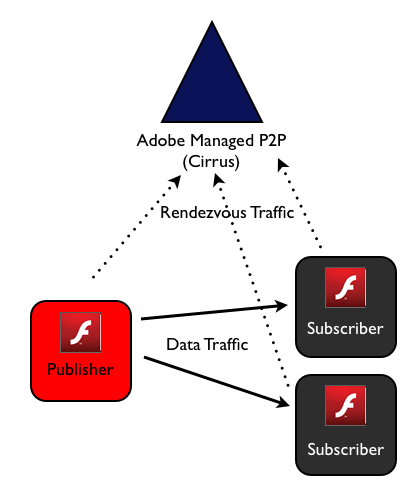
\includegraphics[scale=0.6]{./figures/cirrusAdobe.jpg}
      \caption[RTMFP architecture using Cirrus (source: Adobe)]{RTMFP architecture using Cirrus (source: Adobe).}
	\label{fig:RTMFParchitecture}
\end{figure}
 
Some of the most valuable features is the possibility to easy integrate P2P multicast topologies where one source sends a video to a group of receivers. This is something that none of the other protocols has implemented yet.

\subsection{HTML5}

WebRTC is part of the HTML5 package, both combined are an open cross-platform standard that aims to replace the Adobe proprietary proposal for P2P Real-Time Communication (RTC).

By using HTML5 features we avoid the need of installing any extra software to be able to use real-time multimedia applications on the browser.

\subsubsection{Media Capture and Streams}

HTML5 proposal will replace the existing need to use plugins when having multimedia features in web browsers. This new version carries different API that will be built into the browser and avoid the usage of external software to execute them, this scenario helps to build cross-platform standard applications in JavaScript instead of using plugins. 

Compared with the existing Adobe Flash, APIs such as Web Graphics Library (WebGL) enables developer to build HTML5 3D and 2D games that will work in any browser natively without needing any especial software but with the rendering capabilities of Flash. Mobile browsers have been more likely to adopt this new technology for rendering \cite{webglDraft}. The first final version of the API has been already published and browsers like Chrome and Firefox carry it.

Alongside with WebGL and many other APIs, this new HTML5 also carries the new Media Capture and Streams, also known as GetUserMedia API. This JavaScript API allows developers to access local media such as video/audio from webcams and insert them in a web application by using the new video DOM element \cite{getusermediaDraft}.

This proposal was first attached directly to the WebRTC group but has been published in a different draft, the usage of this API removes the need of using Adobe Flash to access the media device and also the plugin requirement. Developers can capture media streams from cameras and build them into Blob objects to be transmitted to other peers or reproduced locally.

 \begin{figure}[h]
  \centering
    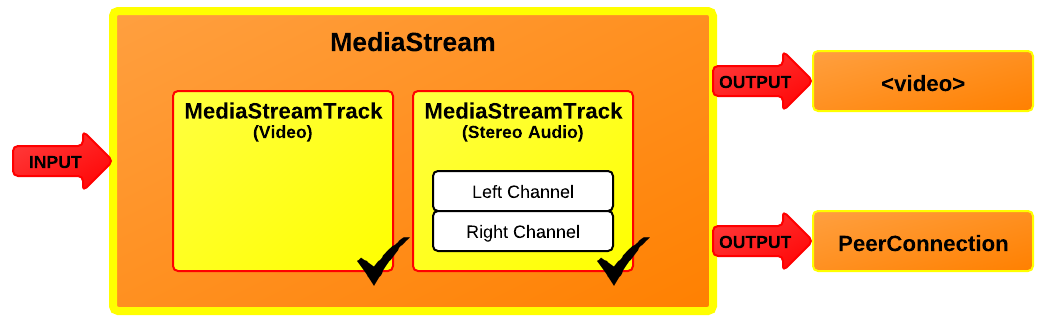
\includegraphics[scale=1]{./figures/mediastreamAPI.png}
      \caption[Media Stream API (source: W3C)]{Media Stream API (source: W3C).}
	\label{fig:mediastreamAPI}
\end{figure}

Figure ~\ref{fig:mediastreamAPI} illustrates how the browser access that media and the outputs delivered to the developer. We will use this function to build WebRTC enabled applications for RTC video conferencing. The video tag is an HTML5 DOM element that reproduces local and remote streams.

\subsubsection{WebRTC}

WebRTC is a working API part of the HTML5 proposal, it is defined in a W3C draft \cite{webrtcW3cgroup}. This API replaces the need of a RTMFP plugin for P2P communications for browsers, WebRTC uses already existing technologies, learned from SIP, bundled into an API. It is able to solve NAT transversal environments by using a mixtures of ICE, TURN and STUN technologies. For the session description it uses a modified bundled version of SDP. The format used for packet transport is RTP and SRTP, modified WebSockets are in use for P2P DataChannel implementation to provide data transport multiplexed over the same stream. All the traffic is sent over UDP or TCP \cite{alvestrandOverview2012}.

This P2P session establishment system works in a constrained environment similar to RTMFP but it has been designed to provide legacy for other SDP based protocols such as SIP. It is a browser side API and does not provide any centralized service for signaling. Figure ~\ref{fig:webrtcExample} shows how a WebRTC simple P2P scenario works, the server used for signaling is based in node.js.

 \begin{figure}[h]
  \centering
    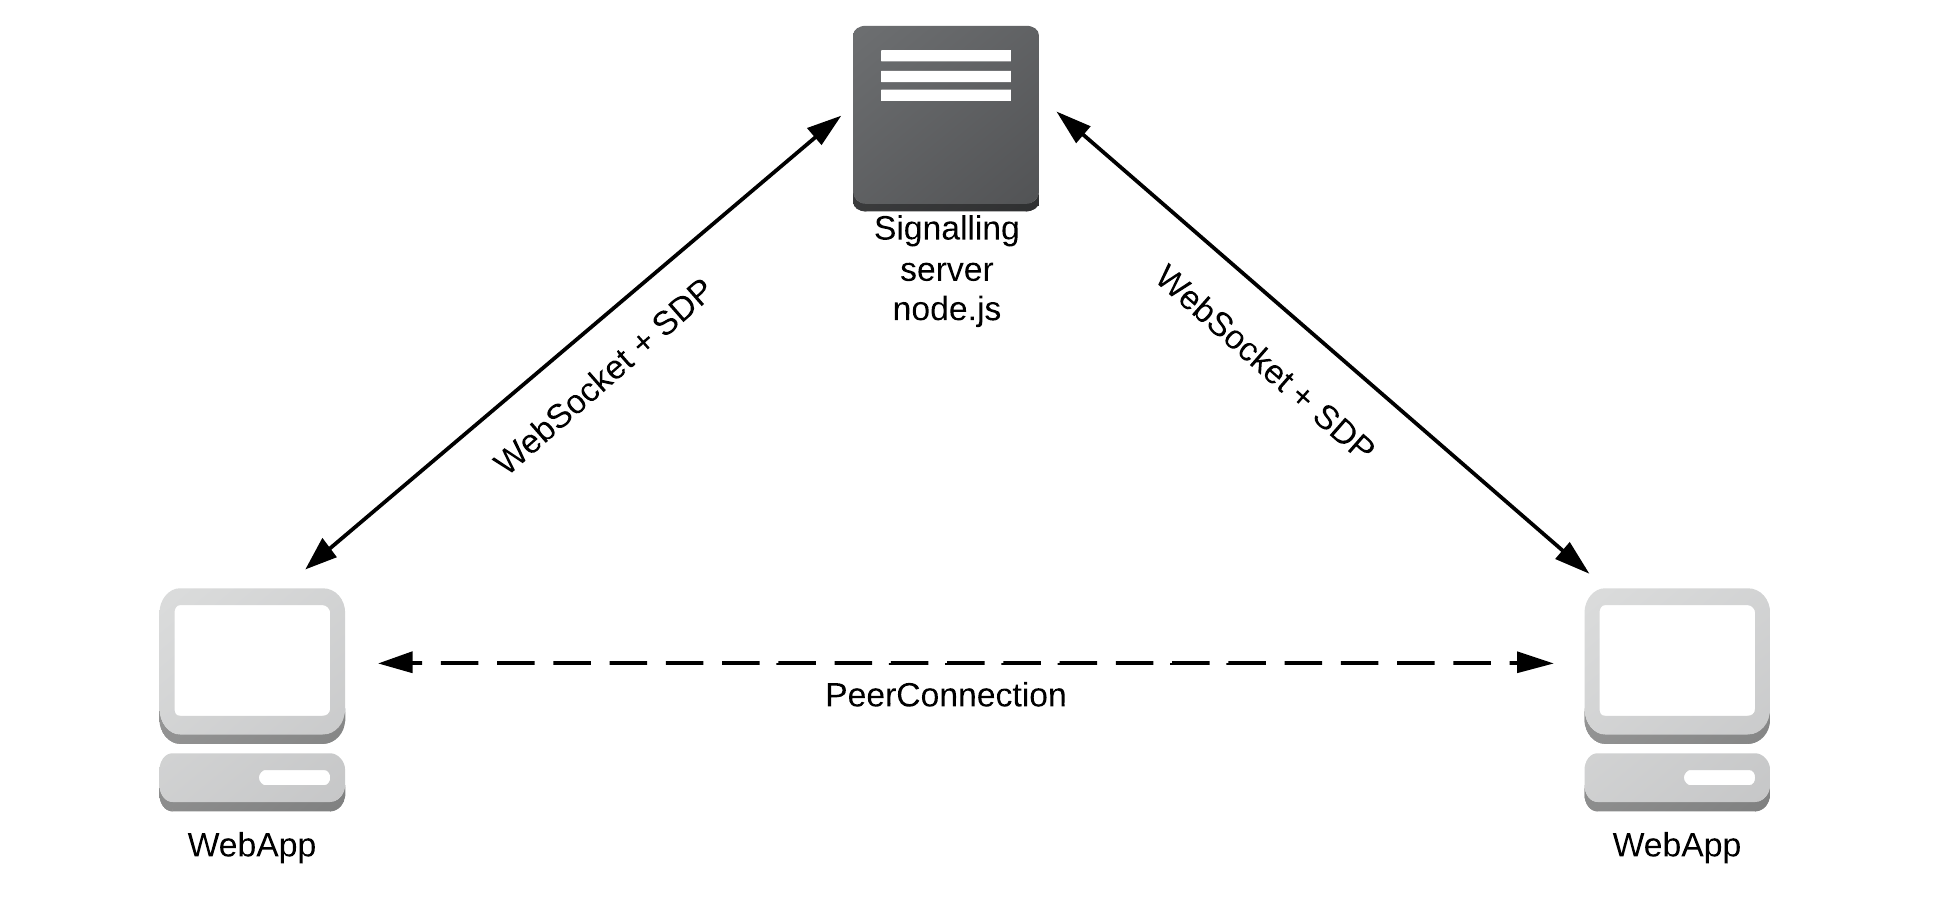
\includegraphics[width=1\textwidth]{./figures/webrtcExample.png}
      \caption[WebRTC simple topology for P2P communication]{WebRTC simple topology for P2P communication.}
	\label{fig:webrtcExample}
\end{figure}

Figure ~\ref{fig:webrtcExample} does not show relay machines that provide NAT transversal solutions, those rely in other technologies that are applied to the API. In this simple example we consider both peers are in the same network without any Firewall or NAT restriction.

\subsection{Issues in WebRTC}

WebRTC uses a mixture of different technologies to perform peer-to-peer communication between clients, those technologies range from SRTP, RTP, RTCP and multiple codecs that are being discussed. This scenario makes performance the key point for success in developing stable WebRTC applications. 

Performance is manly related to computer capabilities and the ability to encode/decode at the same time as transferring and monitoring multiple peer connections. All those tasks are run over the browser and not directly on the OS, this is good for interoperability between platforms but bad in the performance aspect. Compared to Adobe technologies which uses a plugin, the performance they can deliver should be higher as they do not use as many application layers.

Media applications are delay sensitive and require a low packet loss for its proper function, WebRTC is working on this aspect by trying to implement congestion control over the connection stablished between peers, this work is not completed yet and will arise as a problem in the near future. Packet loss due to system capacity and bandwidth are measurable in WebRTC using the Stats API, this API provides information about the PeerConnection performance and is accessible by JavaScript.

Media constraints and bandwidth statistics will make a big difference in how media is acquired in WebRTC. Browsers and web applications have always tolerate some amount of delay and packet losses but this is not possible in media infrastructures for real time applications, an effort is needed to handle Quality of Service (QoS) in WebRTC to compete with RTMFP.

\subsubsection{Quality of Service}

Quality of Service (QoS) for WebRTC is being discussed and an internet draft is available with some proposals \cite{qosWebRTCIETF}. WebRTC uses DiffServ packet marking for QoS but this is not sufficient to help prevent congestion in some environments. Packet marking will help in Wifi and broadband connections but will not be very useful in mobile networks as marking could be removed by the provider. Audio/video packets will be marked as priority using DSCP mappings with audio being more important than video or data \cite{qosWebRTCIETF}. 

The possibility to combine QoS in the transport layer with the constraints and stats of the WebRTC API will help developers to build more adaptive applications, for example, lowing the Frames per Second (FPS) in the case of high packet losses will reduce the bandwidth usage in the case of congestion of the link. This is possible thanks to the Stats API that provide the data statistics for the peer connection.

Some environments will also require better QoS as their bandwidth will be lower, examples in the use case draft relate this to surveillance cameras or similar approaches \cite{WebRTCcasesIETF}. In these cases QoS should be modified by using the API, this situation can lead also to malicious JavaScript injection that could flood the path with packets. 

\subsection{Security concerns}

In order to establish a call in WebRTC we use a web server for the signaling part, on the browser side we rely on built-in standardized JavaScript calling APIs which are used by the web server to establish the call between two peers \cite{WebRTCcasesIETF}. Figure ~\ref{fig:webrtcExample} represents the simple topology for a WebRTC call, even this system is similar to other provided VoIP services, the web server is able to move logic from the JavaScript in the browser giving total control to the server.

Obviously, this system poses a range of new security and privacy challenges different from traditional VoIP systems. It has to avoid malicious calling or having a call established without user knowledge, considering that those APIs are able to bypass Firewalls and NAT, Denial of Services (DoS) attacks are a threat.

Nowadays browsers continuously execute JavaScript codes from accessed web sites, this also includes malicious scripts, but in the case of WebRTC this could lead to a big privacy threat. In a WebRTC environment we consider the browser to be a trusted unit and the JavaScript provided by the server to be unknown as it can execute a variety of actions in the browser. At minimum, it must not be possible for arbitrary sites to initiate calls to arbitrary locations without user consent \cite{rtcwebSecurityIETF}. To approach this, the user must make the decision to allow a call (and the access to its webcam media) with previous knowledge of who is requesting the access, where the media is going or both.

The previous procedure is run by the JavaScript provided by the server, this is a security issue as the user must trust an unknown authority server. Calling services commonly use HTTPS for authentication whose origin can be verified and users should be verified cryptographically (DTLS-SRTP). Browser peers should be authorized before starting the media flow, even this can be done by the PeerConnection itself by using some Identity Provider (IdP) that supports OpenID or BrowserID to demonstrate their identity \cite{rtcwebSecurityArchIETF}. Usually this problem is not particularly important in a closed domain, cases where both peers are in the same social network and provide their profiles to the system and those are exchanged previous to the call, but it arises as a big issue when having federated calls from different domains.

If the web service is running over a trusted HTTPS certificate and has been authenticated it will be possible for the user to set the allow always access to the media, otherwise the user will have to allow this access. Once the media is acquired the actual API builds the ICE candidates for media verification. Authentication and verification in WebRTC is an ongoing discussion in the WG.



%%conclusion chapter
\section{Conclusion}

%% 
%% Leave first page empty
\thispagestyle{empty}

During the development of this thesis we have analyzed and evaluated WebRTC protocol for real-time web applications in different environments. We also compared this protocol with already existing real-time communications alternatives and described the usage of the actual implementation of WebRTC. Furthermore, we also decided a set of key indicators that are important when measuring the performance of a RTC protocol. Those indicators are used when evaluating the congestion control mechanisms of WebRTC. We also described the possible real-time topologies used to test the performance of WebRTC, some of them are still not possible to implement due to API constraints. To evaluate the protocol we also built an specific setup for this thesis, the environment is used during the development of all the thesis. Finally, we executed the tests after describing the proposed congestion control mechanisms and the ones already implemented in WebRTC.

After the tests, we can conclude that WebRTC is a solid protocol for real-time web applications that performs correctly in constrained environments with low latencies, up to 200ms, but cannot hold greater values. This condition may affect mobile applications relying on WebRTC. The congestion control mechanism implemented in WebRTC, Receiver-side Real-time Congestion Control (RRTCC), copes correctly with packet losses protecting the packets with different mechanisms such as Forward Error Correction (FEC). To improve the performance of WebRTC, different congestion control mechanisms that react to other indicators could be implemented in the internals of the browsers.

Furthermore, some future investigations could be done in order to determine the usability limits of WebRTC. Future works include a deeper experience in mobile environments with the two possible implementations: native mobile application and mobile web application. Both are crucial for the expansion of WebRTC into mobile platforms. Besides this, the analysis of WebRTC session on mobile moving nodes is also important to check the response of the call quality.

WebRTC APIs also need enhancements in order to test all possible environments. One of the most interesting areas to investigate, is the development of a transcoding MCU in WebRTC. During this thesis we have used a packet relying MCU environment for the tests, the transcoding MCU multiplexes and mixes the media streams into a unique channel to improve performance over the path. This type of environment is commonly used for multiparty calls. A better understanding of the Stats API implemented in WebRTC is also needed to better adequate the constraints of the media acquisition and the PeerConnection API. Those metrics are provided by the browser internals and can provide valuable feedback for the application developer that can be used to improve the quality of the session.

Lastly, a follow-up of the cross-compatibility of the browser congestion control mechanisms should be studied in order to provide full interoperability between vendors and devices. At the development of this thesis, this compatibility is not achieved due to the lack of congestion control mechanisms in some browser providers.





\addcontentsline{toc}{section}{References}
\bibliographystyle{unsrt}
\bibliography{./chapters/allpapers} 

\end{document}


